\documentclass[compress]{beamer}
\usecolortheme{default}

\usepackage{lmodern, epstopdf, multirow, array, setspace, bbm, tcolorbox, pbox, bm, mathtools, tikz}
\usepackage[T1]{fontenc}

\setbeamertemplate{frametitle}[default][center]
\setbeamertemplate{footline}{\hfill \insertframenumber/\inserttotalframenumber\hspace*{5pt}\vspace{5pt}}
\setbeamertemplate{navigation symbols}{}

\newlength{\wideitemsep}
\setlength{\wideitemsep}{\itemsep}
\addtolength{\wideitemsep}{4pt}
\let\olditem\item
\renewcommand{\item}{\setlength{\itemsep}{\wideitemsep}\olditem}
\setlength{\leftmargini}{12pt}
\setlength{\leftmarginii}{14pt}
\setbeamertemplate{itemize/enumerate subbody begin}{\vspace{6pt}}
\setbeamertemplate{itemize item}[circle]
\setbeamertemplate{enumerate item}[circle]
\setbeamertemplate{enumerate subitem}[default]

\setbeamercolor{alerted text}{fg=blue}
\setbeamersize{text margin left=1.5em,text margin right=1.5em}

\tcbset{
    colback=white,
    colframe=black,
    coltext=black,
    coltitle=blue,
    colbacktitle=white,
    boxrule=1pt,
    titlerule=0pt,
    toptitle=4pt,
    top=2pt
}

\newenvironment{changemargin}[2]{% 
  \begin{list}{}{% 
    \setlength{\topsep}{0pt}% 
    \setlength{\leftmargin}{#1}% 
    \setlength{\rightmargin}{#2}% 
    \setlength{\listparindent}{\parindent}% 
    \setlength{\itemindent}{\parindent}% 
    \setlength{\parsep}{\parskip}% 
  }% 
  \item[]}{\end{list}}
  
\newenvironment{defn}{%
  \begin{tcolorbox}[title={Definition}]%
  }{\end{tcolorbox}}
  
\newenvironment{prop}[1]{%
  \begin{tcolorbox}[title={Proposition #1}]%
  }{\end{tcolorbox}}
  
\newcommand{\cit}[1]{{\footnotesize \textcolor[rgb]{0.5,0,0}{#1}}}

% Font size for code listings (verbatim blocks); reset with \normalsize
\newcommand{\codesize}{\fontsize{7}{8.5}\selectfont}

\newcommand{\slidesetup}[1]{%
  \title{#1}%
  \subtitle{\texorpdfstring{\vspace{0.3\baselineskip}}{} {\small This version: \today}}%
  \author[Mikkel Plagborg-Moller]{ECMA 31150, Spring 2026 \texorpdfstring{\\[0.5ex]}{} University of Chicago \texorpdfstring{\\[0.5ex]}{} Department of Economics \texorpdfstring{\\[4ex]}{} Mikkel Plagborg-Moller}%
  \date{}%
}

% \circleoverlay[options]{text}
% Draws a red circle with a text box nearby on a tikz overlay.
% Options (with defaults):
%   cx=0cm, cy=0cm      - circle center (shift from page center)
%   r=1cm               - circle radius
%   tx=0cm, ty=0cm      - text box offset from circle center
%   text anchor=east    - anchor of text node (east = text left, west = text right)
%   font=\normalsize    - font size for text
\pgfkeys{
  /circleoverlay/.cd,
  cx/.store in=\cocx, cx=0cm,
  cy/.store in=\cocy, cy=0cm,
  r/.store in=\cor, r=1cm,
  tx/.store in=\cotx, tx=0cm,
  ty/.store in=\coty, ty=0cm,
  text anchor/.store in=\cotextanchor, text anchor=east,
  font/.store in=\cofont, font=\normalsize,
}
\newcommand{\circleoverlay}[2][]{%
  \pgfkeys{/circleoverlay/.cd, cx=0cm, cy=0cm, r=1cm, tx=0cm, ty=0cm, text anchor=east, font=\normalsize, #1}%
  \pgfmathsetlengthmacro{\circlediameter}{2*\cor}%
  \node[draw=red, line width=2pt, circle, minimum size=\circlediameter, inner sep=0pt]
    (tmpcirc) at ([xshift=\cocx,yshift=\cocy]current page.center) {};%
  \node[anchor=\cotextanchor, fill=white, draw=red, text=red, inner sep=4pt, align=left, font=\cofont]
    at ([xshift=\cotx,yshift=\coty]tmpcirc.center) {#2};%
}

\DeclareMathOperator*{\argmax}{argmax}
\DeclareMathOperator*{\argmin}{argmin}
\DeclareMathOperator{\diag}{diag}
\DeclareMathOperator{\var}{Var}
\DeclareMathOperator{\cov}{Cov}
\DeclareMathOperator{\corr}{Corr}
\DeclareMathOperator{\lrv}{LRV}

\usepackage{pifont}

\slidesetup{Dynamic causal effects I}

\begin{document}
\frame{
\maketitle
}

\frame{
\frametitle{Plan for this slide deck}
\begin{enumerate}
\item Dynamic causal effects
\begin{itemize}
\item Rules vs.\ shocks
\item Impulse response functions
\end{itemize}
\item Local projections with observed shock
\begin{itemize}
\item Control variables, lag length selection
\item Standard errors, confidence band
\end{itemize}
\item Identification from timing restrictions
\end{enumerate}
}

\frame{
\frametitle{Causal inference in macroeconomics}
\begin{itemize}
\item Classic question: how does monetary policy affect the real economy?
\item In most countries outside crisis periods, monetary policy operates by manipulating short-term interest rates (U.S.: federal funds rate).
\item A simple regression of GDP growth on short-term interest rates does not estimate a causal effect.
\begin{itemize}
\item Simultaneous causality: policy-makers set the interest rate in response to economic developments.
\end{itemize}
\item Even if, hypothetically, monetary policy-makers did not pay attention to the economy, we'd still need to distinguish between two types of interest rate changes with disparate causal effects:
\begin{enumerate}
\item Anticipated changes.
\item Unanticipated changes: \textbf{shocks}.
\end{enumerate}
\end{itemize}
}

\frame{
\frametitle{Causal inference in macroeconomics (cont.)}
\begin{itemize}
\item Example: suppose policy-makers choose the interest rate according to a \textbf{Taylor rule}
\[i_t = \underbrace{c + \phi_i i_{t-1} + \phi_\pi \pi_t + \phi_y y_t}_\text{systematic \textbf{policy rule}} +\; \varepsilon_t.\]
\vspace{-1.3\baselineskip}
\begin{itemize}
\item $i_t$: nominal interest rate
\item $\pi_t$: inflation
\item $y_t$: output
\item $\varepsilon_t$: monetary policy shock (idiosyncratic deviation from rule)
\end{itemize}
\item Two-way feedback: $i_t \leftrightarrow (\pi_t,y_t)$.
\end{itemize}
}

\frame{
\frametitle{Causal inference in macroeconomics (cont.)}
\[i_t = c + \phi_i i_{t-1} + \phi_\pi \pi_t + \phi_y y_t + \varepsilon_t\]
\begin{itemize}
\item Consider a change to the systematic policy rule (e.g., increasing $\phi_i$).
\begin{itemize}
\item Economic agents \textbf{anticipate} a new equilibrium even in the long run.
\item Agents fundamentally change their behavior (e.g., their formula for forecasting the future).
\end{itemize}
\item Now consider a one-off surprise change to $\varepsilon_t$ (a shock).
\begin{itemize}
\item Agents update expectations about short-run economic conditions, but the structure of the economy is unchanged.
\end{itemize}
\item The causal effects of these two types of changes are not the same.
\end{itemize}
}

\frame{
\frametitle{Causal inference in macroeconomics (cont.)}
\begin{itemize}
\item In practice, we do not cleanly observe many structural changes in policy rules in historical data. Difficult (but not impossible) to estimate causal effects of changing the policy \emph{rule}.
\item Instead we will focus on estimating causal effects of \emph{shocks}: deviations from the policy rule.
\item Where do policy shocks come from?
\begin{itemize}
\item Idiosyncratic preferences of rotating cast of policy-makers (e.g., inflation hawks/doves).
\item One-off political events.
\item Private information of policy-makers.
\item Desire to surprise markets (but can't do this all the time).
\end{itemize}
\end{itemize}
\medskip
\begin{quotation}
You can fool some people sometimes, but you can't fool all the people all the time. 
\hfill --- {\upshape Bob Marley}
\end{quotation}
}

\frame{
\frametitle{Structural vector moving average model}
\begin{itemize}
\item Let $y_t$ be an observed macro time series.
\begin{itemize}
\item GDP, inflation, interest rate, etc.
\end{itemize}
\item Let $\bm{\varepsilon}_t$ be an $n_\varepsilon \times 1$ vector of potentially unobserved shocks.
\item \textbf{Structural vector moving average} (SVMA) model:
\[y_t = \mu + \bm{\Theta}_0 \bm{\varepsilon}_t + \bm{\Theta}_1 \bm{\varepsilon}_{t-1} + \bm{\Theta}_2 \bm{\varepsilon}_{t-2} + \dots = \mu + \bm{\Theta}(L)\bm{\varepsilon}_t,\]
where $\bm{\Theta}(L) = \sum_{\ell=0}^\infty \bm{\Theta}_\ell L^\ell$ is of dimension $1 \times n_\varepsilon$.
\end{itemize}
}

\frame{
\frametitle{Structural vector moving average model (cont.)}
\begin{itemize}
\item The observed variable can depend on all lags of all shocks:
\[y_t = \mu + \sum_{j=1}^{n_\varepsilon} \sum_{\ell=0}^\infty \Theta_{\ell j} \varepsilon_{j,t-\ell}.\]
\vspace{-\baselineskip}
\begin{itemize}
\item $\Theta_{\ell j}$: $j$-th element of $\bm{\Theta}_\ell$.
\end{itemize}
\item Apart from linearity, SVMA model places \emph{no restrictions} on the \textbf{propagation mechanism} from shocks to observed macro outcomes.
\item Encompasses any linear theoretical macro model you can think of.
\begin{itemize}
\item \alert{Exercise:} if $y_t=c+\rho y_{t-1} + \varepsilon_t$ with $|\rho|<1$, how can you represent $y_t$ in SVMA form?
\end{itemize}
\end{itemize}
}

\frame{
\frametitle{Structural vector moving average model: shocks}
\[y_t = \mu + \bm{\Theta}_0 \bm{\varepsilon}_t + \bm{\Theta}_1 \bm{\varepsilon}_{t-1} + \bm{\Theta}_2 \bm{\varepsilon}_{t-2} + \dots = \mu +  \bm{\Theta}(L)\bm{\varepsilon}_t\]
\vspace{-0.5\baselineskip}
\begin{itemize}
\item Consistent with our earlier discussion, we assume that shocks are serially uncorrelated: $\bm{\varepsilon}_t \sim \mathit{WN}(\bm{D})$.
\begin{itemize}
\item A ``shock'' has to be unpredictable from past information.
\end{itemize}
\item Moreover, we assume that the variance-covariance matrix $\bm{D}$ is diagonal, so shocks are \textbf{mutually uncorrelated}:
\[\bm{D} = \diag(\sigma_1^2,\sigma_2^2,\dots,\sigma_{n_\varepsilon}^2) \quad \Longrightarrow \quad E[\varepsilon_{it}\varepsilon_{jt}]=0 \quad \text{for } i \neq j.\]
\vspace{-1.3\baselineskip}
\begin{itemize}
\item Different shocks correspond to conceptually distinct external forces that drive the economy (monetary policy, technology, climate, etc.).
\item If two supposed ``shocks'' were correlated, they should be viewed as both being caused by a third, more fundamental shock.
\end{itemize}
\end{itemize}
}

\frame{
\frametitle{Structural vector moving average model (cont.)}
\[y_t = \mu + \bm{\Theta}(L)\bm{\varepsilon}_t,\quad \bm{\varepsilon}_t \sim \mathit{WN}(\bm{D}),\quad \bm{D} = \diag(\sigma_1^2,\sigma_2^2,\dots,\sigma_{n_\varepsilon}^2)\]
\begin{itemize}
\item SVMA model casts the Frisch-Slutsky-Yule \textbf{impulse-propagation framework} as a causal model (recall our first lecture).
\item Meaningful to think of manipulating one shock while holding all other shocks constant.
\item Presumably, there are in reality thousands of different kinds of shocks that drive the economy (not just policy, but also surprise changes to economic fundamentals such as technology).
\end{itemize}
}

\frame{
\frametitle{SVMA: impulse response function}
\begin{itemize}
\item How does a shock, say the first one $\varepsilon_{1t}$, causally affect the outcomes now and in the future: $y_t$, $y_{t+1}$, $y_{t+2}$, \dots?
\item Let $h \geq 0$. Let's express $y_{t+h}$ as a function of $\varepsilon_{1t}$ plus other stuff:
\begin{align*}
y_{t+h} &= \mu + \sum_{j=1}^{n_\varepsilon} \sum_{\ell=0}^\infty \Theta_{\ell j} \varepsilon_{j,t+h-\ell} \\
&= \mu + \Theta_{0\alert{1}} \varepsilon_{\alert{1},t+h} + \Theta_{1\alert{1}} \varepsilon_{\alert{1},t+h-1} + \Theta_{2\alert{1}} \varepsilon_{\alert{1},t+h-2} + \dots \\
&\qquad + \sum_{j=\alert{2}}^{n_\varepsilon} \sum_{\ell=0}^\infty \Theta_{\ell j} \varepsilon_{j,t+h-\ell} \\
&= \mu + \alert{\Theta_{h1}\varepsilon_{1t}} + \sum_{\alert{\ell \neq h}} \Theta_{\ell 1} \varepsilon_{1,t+h-\ell} + \sum_{j=\alert{2}}^{n_\varepsilon} \sum_{\ell=0}^\infty \Theta_{\ell j} \varepsilon_{j,t+h-\ell}.
\end{align*}
\item Causal effect on $y_{t+h}$ of increasing $\varepsilon_{1t}$ by 1 unit: $\boxed{\Theta_{h1}}$.
\end{itemize}
}

\frame{
\frametitle{SVMA: impulse response function (cont.)}
\begin{itemize}
\item If $\varepsilon_{1t}$ is increased by 1 unit, holding everything else constant (including past and future shocks)\dots
\begin{itemize}
\item Current period (\textbf{on impact}): $y_t$ changes by $\Theta_{01}$.
\item Next period: $y_{t+1}$ changes by $\Theta_{11}$.
\item Two periods in the future: $y_{t+2}$ changes by $\Theta_{21}$\dots
\end{itemize}
\item The MA parameter $\Theta_{h1}$ is called the \textbf{impulse response} at \textbf{horizon} $h$.
\item We call $(\Theta_{01},\Theta_{11},\Theta_{21},\dots)$ the \textbf{impulse response function} (IRF) -- or \textbf{dynamic causal effects} -- of $\lbrace y_t \rbrace$ with respect to the shock $\lbrace \varepsilon_{1t} \rbrace$.
\end{itemize}
}

\frame{
\frametitle{Impulse response function: examples}
\begin{itemize}
\item SVMA(2) model:
\[y_t = \varepsilon_{1t} - 0.5\varepsilon_{1,t-1} + \varepsilon_{2,t-1} + 0.2\varepsilon_{1,t-2}\]
\vspace{-1.5\baselineskip}
\begin{itemize}
\item IRF of $y_t$ wrt.\ $\varepsilon_{1t}$: $(1, -0.5, 0.2, 0, 0, \dots)$.
\item IRF of $y_t$ wrt.\ $\varepsilon_{2t}$: $(0, 1, 0, 0, 0, \dots)$.
\end{itemize}
\medskip
\item \alert{Exercise:} show that in the AR(1) model $y_t = c + \rho y_{t-1} + \varepsilon_t$, the IRF of $y_t$ wrt.\ $\varepsilon_t$ is $(1, \rho, \rho^2, \rho^3, \dots)$.
\end{itemize}
}

\frame{
\frametitle{Impulse response function: estimation}
\begin{itemize}
\item Suppose we directly measure the shock $\varepsilon_{1t}$.
\item From our earlier derivation:
\[y_{t+h} = \mu + \alert{\Theta_{h1}\varepsilon_{1t}} + \underbrace{\sum_{\alert{\ell \neq h}} \Theta_{\ell 1} \varepsilon_{1,t+h-\ell} + \sum_{j=\alert{2}}^{n_\varepsilon} \sum_{\ell=0}^\infty \Theta_{\ell j} \varepsilon_{j,t+h-\ell}}_{\equiv v_{h,t+h}}.\]
\item By our assumptions on the shocks, $\varepsilon_{1t}$ is uncorrelated with each of the terms that appear in $v_{h,t+h}$:
\[E[\varepsilon_{1t}\varepsilon_{j,t+h-\ell}]=0 \quad \text{if either } j \neq 1 \text{ or } \ell \neq h.\]
\item We can therefore consistently estimate the impulse response $\Theta_{h1}$ through an OLS regression of $y_{t+h}$ on $\varepsilon_{1t}$.
\item Notation: to emphasize that $\varepsilon_{1t}$ is observed, I will call it $x_t$.
\end{itemize}
}

\frame{
\frametitle{Local projections}
\begin{itemize}
\item Separately for each horizon $h=0,1,\dots,h_{\max}$ of interest, we run an OLS regression
\[y_{t+h} = \hat{c}_h + \hat{\beta}_h x_t + \hat{v}_{h,t+h}.\]
\item Then $\hat{\beta}_h$ consistently estimates the impulse response $\Theta_{h1}$. The estimated IRF up to horizon $h_{\max}$ is $(\hat{\beta}_0,\hat{\beta}_1,\dots,\hat{\beta}_{h_{\max}})$.
\item These regressions are called \textbf{local projections} (LPs).
\item We could do this for different macro observables $y_t$.
\item The true regression error term $v_{h,t+h}$ is serially correlated, which suggests reporting Newey-West SE (more on this later).
\end{itemize}
}

\frame{
\begin{figure}
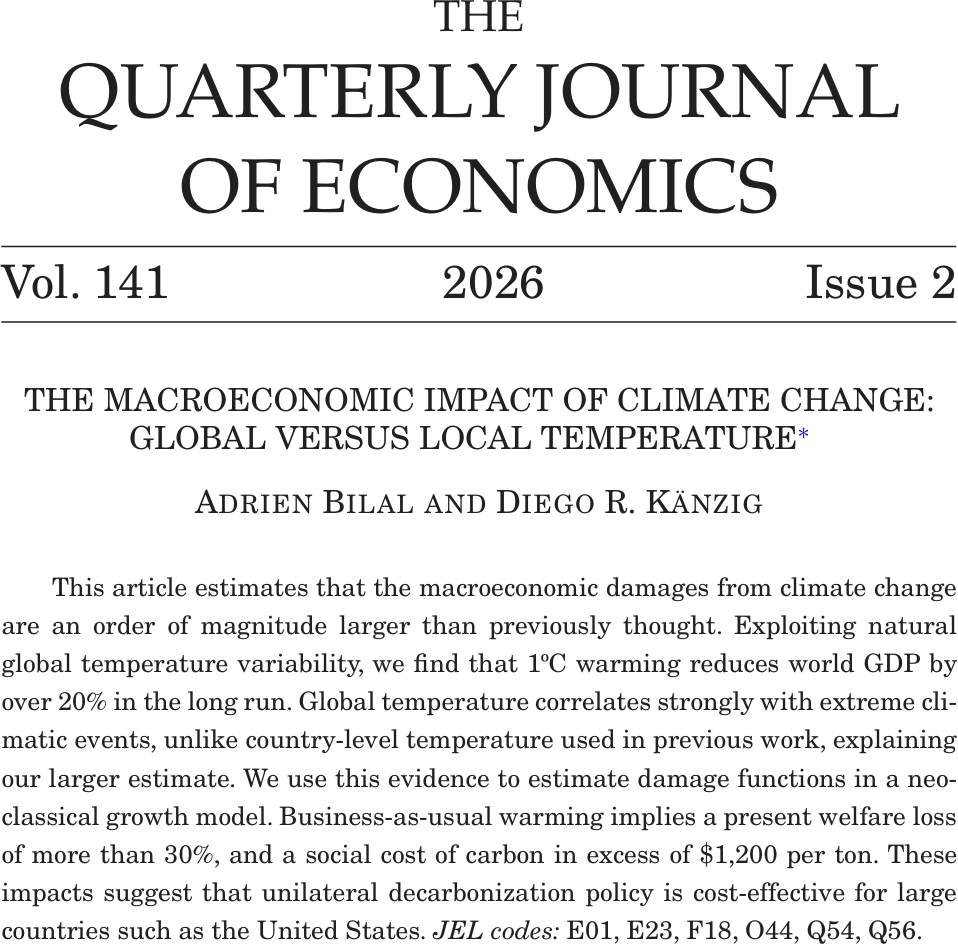
\includegraphics[width=0.7\linewidth]{fig/bk2026.png}
\end{figure}
}

\frame{
\begin{figure}
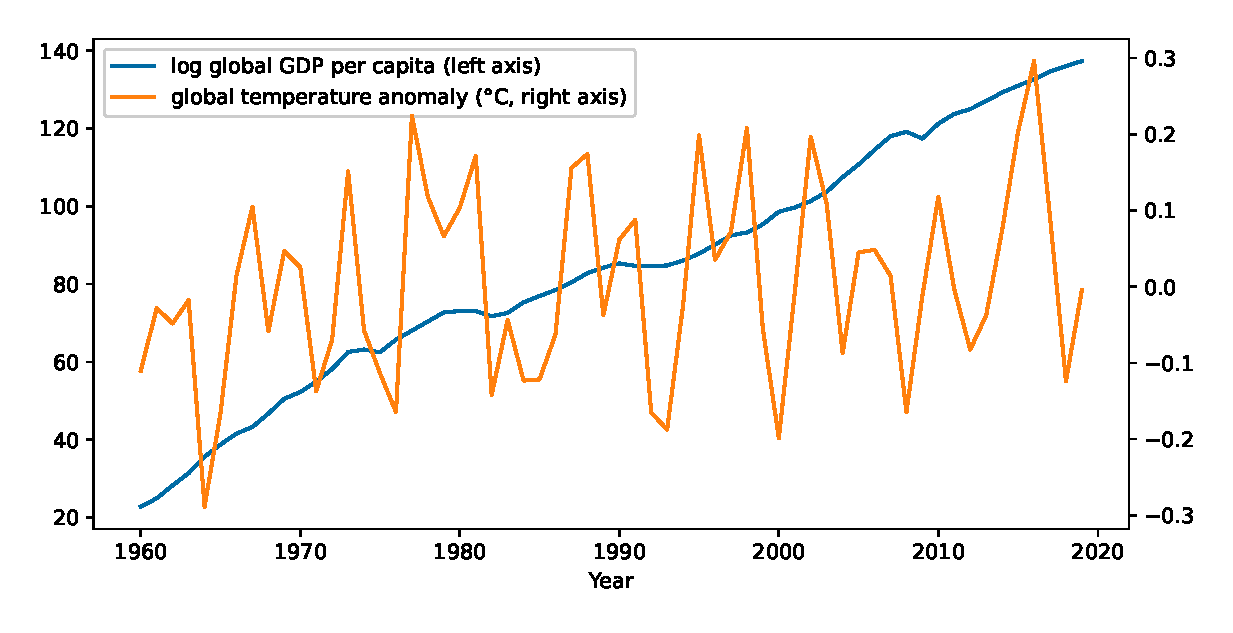
\includegraphics[width=\linewidth]{fig/bk_gdp_temp.eps} \\
\smallskip
Temperature anomaly: deviation of global temperature from medium-run trend
\end{figure}
}

\begin{frame}[fragile]
\scriptsize
\begin{verbatim}
max_horizon = 10
T = df[['l_gdp', 'temp_anom']].dropna().shape[0]
nw_bw = int(np.ceil(0.75 * T**(1/3)))

irf = np.empty(max_horizon + 1)
se  = np.empty(max_horizon + 1)
for h in range(max_horizon + 1):
    y = (df['l_gdp'].shift(-h) - df['l_gdp'].shift(1)).rename(f'dl_gdp_h{h}')
    X = sm.add_constant(df[['temp_anom']])
    reg = sm.OLS(y, X, missing='drop').fit(
        cov_type='HAC', cov_kwds={'maxlags': nw_bw - 1}
        )
    irf[h] = reg.params['temp_anom']
    se[h]  = reg.bse['temp_anom']
\end{verbatim}
\medskip
\normalsize
\begin{itemize}
\item Note: since GDP has a clear upward trend over time, I transform the dependent variable in the regression to ``long differences'' $y_{t+h}-y_{t-1}$, which look more stationary.
\item The long differences $(y_{t} - y_{t-1}),(y_{t+1} - y_{t-1}),(y_{t+2} - y_{t-1}),\dots$ are labeled \texttt{dl\_gdp\_h0}, \texttt{dl\_gdp\_h1}, \texttt{dl\_gdp\_h2}, \dots
\end{itemize}
\end{frame}

\begin{frame}[fragile]
\scriptsize
\begin{verbatim}
                            OLS Regression Results                            
==============================================================================
Dep. Variable:              dl_gdp_h0   R-squared:                       0.000
Model:                            OLS   Adj. R-squared:                 -0.017
Method:                 Least Squares   F-statistic:                  0.004007
Date:                Wed, 22 Apr 2026   Prob (F-statistic):              0.950
Time:                        13:19:42   Log-Likelihood:                -100.84
No. Observations:                  59   AIC:                             205.7
Df Residuals:                      57   BIC:                             209.8
Df Model:                           1                                         
Covariance Type:                  HAC                                         
==============================================================================
                 coef    std err          z      P>|z|      [0.025      0.975]
------------------------------------------------------------------------------
const          1.9419      0.217      8.936      0.000       1.516       2.368
temp_anom     -0.0936      1.479     -0.063      0.950      -2.992       2.805
==============================================================================
Omnibus:                        3.905   Durbin-Watson:                   1.268
Prob(Omnibus):                  0.142   Jarque-Bera (JB):                3.212
Skew:                          -0.565   Prob(JB):                        0.201
Kurtosis:                       3.176   Cond. No.                         8.02
==============================================================================

Notes:
[1] Standard Errors are heteroscedasticity and autocorrelation robust (HAC)
using 2 lags and without small sample correction
\end{verbatim}
\begin{tikzpicture}[overlay, remember picture]
  \circleoverlay[cx=-1cm, cy=3.75cm, r=0.8cm,
                 tx=-1cm, ty=0.5cm, text anchor=east]{$h=0$}
  \circleoverlay[cx=-3.2cm, cy=-0.6cm, r=0.6cm,
                 tx=0.8cm, ty=-1.2cm, text anchor=south]{$\hat{\beta}_0$}
\end{tikzpicture}
\end{frame}

\begin{frame}[fragile]
\scriptsize
\begin{verbatim}
                            OLS Regression Results                            
==============================================================================
Dep. Variable:              dl_gdp_h1   R-squared:                       0.002
Model:                            OLS   Adj. R-squared:                 -0.016
Method:                 Least Squares   F-statistic:                   0.08369
Date:                Wed, 22 Apr 2026   Prob (F-statistic):              0.773
Time:                        13:19:42   Log-Likelihood:                -128.62
No. Observations:                  58   AIC:                             261.2
Df Residuals:                      56   BIC:                             265.4
Df Model:                           1                                         
Covariance Type:                  HAC                                         
==============================================================================
                 coef    std err          z      P>|z|      [0.025      0.975]
------------------------------------------------------------------------------
const          3.8956      0.414      9.418      0.000       3.085       4.706
temp_anom     -0.7030      2.430     -0.289      0.772      -5.465       4.059
==============================================================================
Omnibus:                        2.629   Durbin-Watson:                   0.721
Prob(Omnibus):                  0.269   Jarque-Bera (JB):                2.500
Skew:                          -0.491   Prob(JB):                        0.286
Kurtosis:                       2.732   Cond. No.                         7.96
==============================================================================

Notes:
[1] Standard Errors are heteroscedasticity and autocorrelation robust (HAC)
using 2 lags and without small sample correction
\end{verbatim}
\begin{tikzpicture}[overlay, remember picture]
  \circleoverlay[cx=-1cm, cy=3.75cm, r=0.8cm,
                 tx=-1cm, ty=0.5cm, text anchor=east]{$h=1$}
  \circleoverlay[cx=-3.2cm, cy=-0.6cm, r=0.6cm,
                 tx=0.8cm, ty=-1.2cm, text anchor=south]{$\hat{\beta}_1$}
\end{tikzpicture}
\end{frame}

\begin{frame}[fragile]
\scriptsize
\begin{verbatim}
                            OLS Regression Results                            
==============================================================================
Dep. Variable:              dl_gdp_h2   R-squared:                       0.017
Model:                            OLS   Adj. R-squared:                 -0.000
Method:                 Least Squares   F-statistic:                     1.068
Date:                Wed, 22 Apr 2026   Prob (F-statistic):              0.306
Time:                        13:19:42   Log-Likelihood:                -140.40
No. Observations:                  57   AIC:                             284.8
Df Residuals:                      55   BIC:                             288.9
Df Model:                           1                                         
Covariance Type:                  HAC                                         
==============================================================================
                 coef    std err          z      P>|z|      [0.025      0.975]
------------------------------------------------------------------------------
const          5.8527      0.577     10.140      0.000       4.721       6.984
temp_anom     -3.0120      2.914     -1.034      0.301      -8.723       2.699
==============================================================================
Omnibus:                        1.677   Durbin-Watson:                   0.418
Prob(Omnibus):                  0.432   Jarque-Bera (JB):                1.664
Skew:                          -0.375   Prob(JB):                        0.435
Kurtosis:                       2.628   Cond. No.                         7.96
==============================================================================

Notes:
[1] Standard Errors are heteroscedasticity and autocorrelation robust (HAC)
using 2 lags and without small sample correction
\end{verbatim}
\begin{tikzpicture}[overlay, remember picture]
  \circleoverlay[cx=-1cm, cy=3.75cm, r=0.8cm,
                 tx=-1cm, ty=0.5cm, text anchor=east]{$h=2$}
  \circleoverlay[cx=-3.2cm, cy=-0.6cm, r=0.6cm,
                 tx=0.8cm, ty=-1.2cm, text anchor=south]{$\hat{\beta}_2$}
\end{tikzpicture}
\end{frame}

\frame{
\begin{figure}
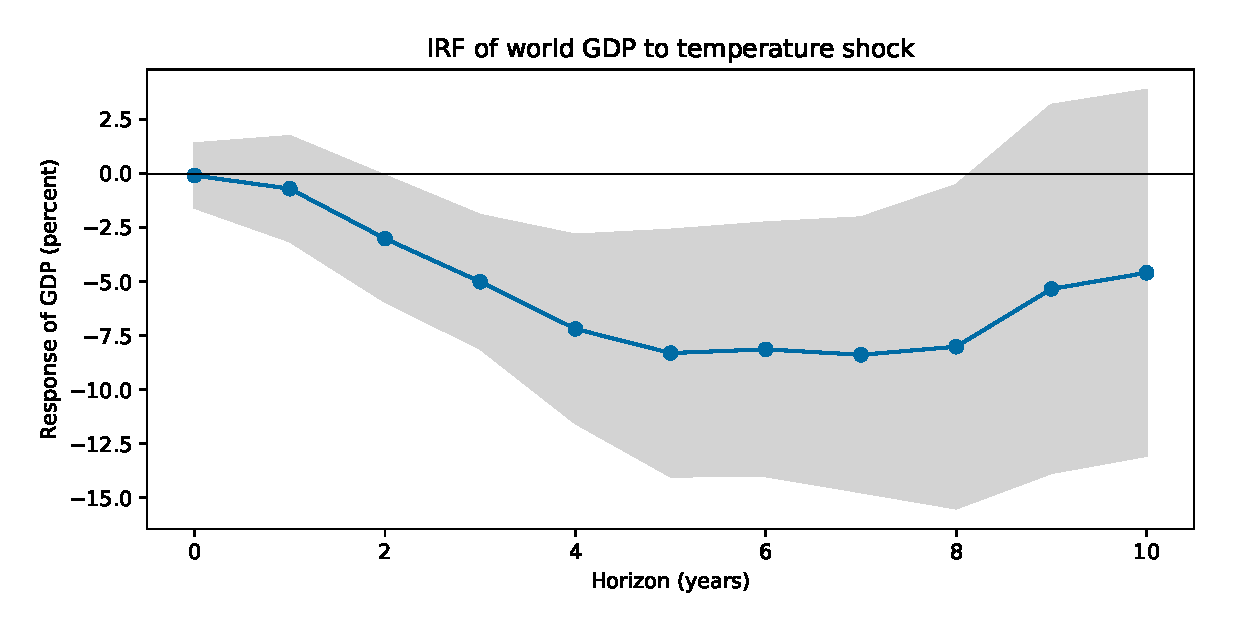
\includegraphics[width=\linewidth]{fig/bk_irf_nocontrols.eps} \\
\medskip
Blue dots: estimated IRF \\[0.5\baselineskip]
Grey region: 68\% \textbf{confidence band} formed by the collection of 68\% confidence intervals for each of the impulse responses
\end{figure}
}

\frame{
\frametitle{Control variables}
\begin{itemize}
\item The LP estimator is consistent under our assumptions. But we can obtain more \emph{efficient} estimates by controlling for lagged variables in our regressions:
\[y_{t+h} = \hat{c}_h + \hat{\beta}_h x_t + \hat{\bm{\delta}}_1'\bm{w}_{t-1} + \dots + \hat{\bm{\delta}}_p'\bm{w}_{t-p} + \hat{v}_{h,t+h},\]
where $\bm{w}_t$ is a vector of data series (including $y_t$, $x_t$, and potentially other variables).
\item If $x_t=\varepsilon_{1t}$ is a shock, it's uncorrelated with $\bm{w}_{t-1},\dots,\bm{w}_{t-p}$, so the controls are not needed to remove omitted variable bias.
\item But the controls ``soak up'' part of the variance of the regression residual, which leads to smaller SE.
\end{itemize}
}

\frame{
\frametitle{Control variables and SE}
\[y_{t+h} = \hat{c}_h + \hat{\beta}_h x_t + \hat{\bm{\delta}}_1'\bm{w}_{t-1} + \dots + \hat{\bm{\delta}}_p'\bm{w}_{t-p} + \hat{v}_{h,t+h}\]
\vspace{-0.5\baselineskip}
\begin{itemize}
\item In fact, it can be shown that, under some reasonable assumptions, if we control for enough variables in $\bm{w}_t$ and enough lags $p$, then we can use heteroskedasticity-robust SE for $\hat{\beta}_h$ rather than Newey-West.
\begin{itemize}
\item Simulations show that the former SE typically work better in finite samples. Moreover, they do not require choosing a bandwidth.
\item Though $\lbrace v_{h,t+h} \rbrace$ is serially correlated, the product $\lbrace x_t \times v_{h,t+h} \rbrace$ is typically much less so if $x_t$ is a shock. Recall that it's the LRV of the product process that matters for SE.
\end{itemize}
\item Should control for variables that are strong predictors of $y_t$.
\item Can select $p$ using AIC applied to a VAR in all the variables in the regression.
\end{itemize}
}

\begin{frame}[fragile]
\footnotesize
\begin{verbatim}
controls = ['l_gdp', 'temp_anom', 'lnpoil_wti',
            'treasury1y', 'recessiondates']
var_model = sm.tsa.VAR(df[controls].dropna())
lag_order = var_model.select_order(maxlags=4)
print(lag_order.summary())
\end{verbatim}
\bigskip
\normalsize

\textbf{Results:}
\footnotesize
\begin{verbatim}
VAR Order Selection (* highlights the minimums) 
=================================================
      AIC         BIC         FPE         HQIC   
-------------------------------------------------
0       9.783       9.964   1.773e+04       9.853
1     0.5904*      1.675*      1.812*      1.011*
2      0.6255       2.615       1.918       1.397
3      0.8745       3.768       2.602       1.996
4      0.9227       4.720       3.050       2.395
-------------------------------------------------
\end{verbatim}
\smallskip
\normalsize
I'll use $p=2$ to be on the safe side.
\end{frame}

\begin{frame}[fragile]
\footnotesize
\begin{verbatim}
def local_projection(df, outcome, shock, controls, max_horz):
    """Local projection IRF with SE"""
    irf = np.empty(max_horz + 1)
    se  = np.empty(max_horz + 1)
    for h in range(max_horz + 1):
        y = df[outcome].shift(-h)
        X = sm.add_constant(df[[shock] + controls])
        reg = sm.OLS(y, X, missing='drop').fit(cov_type='HC1')
        irf[h] = reg.params[shock]
        se[h]  = reg.bse[shock]
    return irf, se
\end{verbatim}
\end{frame}

\begin{frame}[fragile]
\scriptsize
\begin{verbatim}
# Create lagged data
nlag = 2
df = df.assign(**{
    f'{var}_lag{l}': df[var].shift(l)
    for var in controls for l in range(1, nlag + 1)
})
lag_cols = [f'{var}_lag{l}' for var in controls for l in range(1, nlag + 1)]

# LP with lagged controls
irf, se = local_projection(df, 'l_gdp', 'temp_anom', lag_cols, max_horizon)
\end{verbatim}
\bigskip
\small
Note: the outcome can now just be $y_{t+h}$ rather than $(y_{t+h}-y_{t-1})$, since the long differencing is absorbed by the lagged control $y_{t-1}$. Effectively, this lagged control removes any trend in the outcome.
\end{frame}

\frame{
\begin{figure}
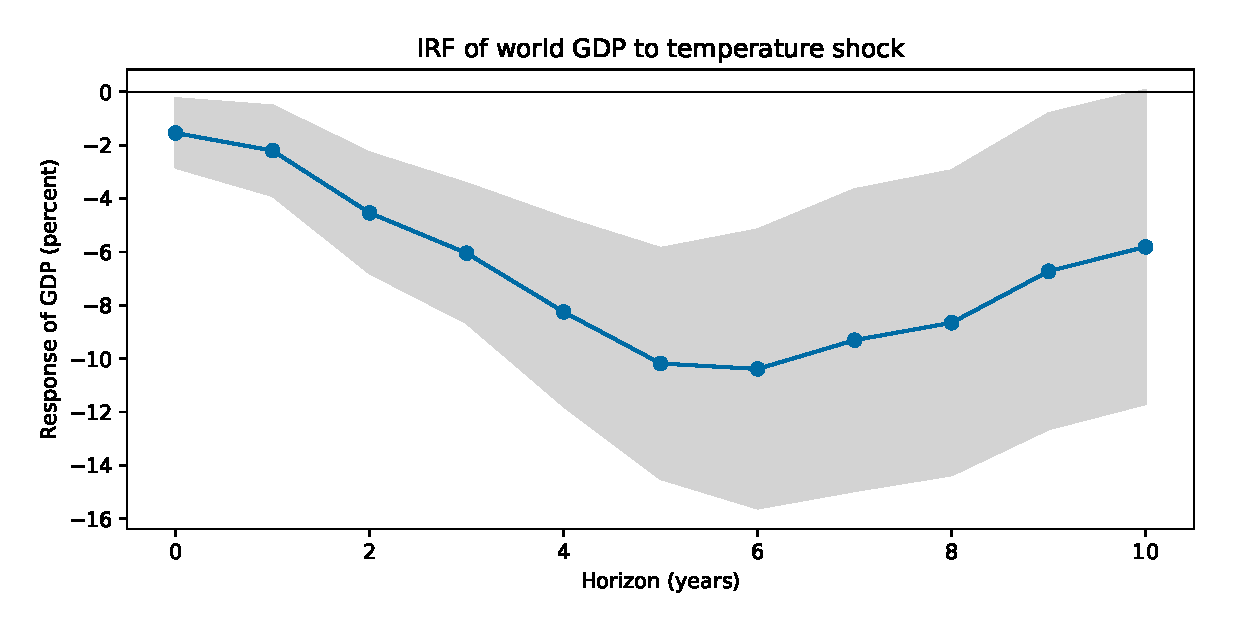
\includegraphics[width=\linewidth]{fig/bk_irf_controls.eps} \\
\bigskip
Controls: 2 lags of outcome, shock, oil price, 1-year Treasury rate, global recession indicator \\
\medskip
The confidence band is narrower than w/o controls -- increased efficiency! \\
\end{figure}
}

\frame{
\frametitle{Is the ``shock'' a shock?}
\begin{itemize}
\item $x_t$ is supposed to be a shock, and thus unpredictable.
\item We can test this by regressing this supposed shock on lagged data (including lags of itself).
\item In the application, we should be worried: the IRF estimates changed quite a bit when we added lagged controls, even though $x_t$ ought to be uncorrelated with those lags.
\end{itemize}
}

\begin{frame}[fragile]
\tiny
\begin{verbatim}
                            OLS Regression Results                            
==============================================================================
Dep. Variable:              temp_anom   R-squared:                       0.155
Model:                            OLS   Adj. R-squared:                  0.074
Method:                 Least Squares   F-statistic:                     2.486
Date:                Tue, 21 Apr 2026   Prob (F-statistic):             0.0430
Time:                        09:23:44   Log-Likelihood:                 42.917
No. Observations:                  58   AIC:                            -73.83
Df Residuals:                      52   BIC:                            -61.47
Df Model:                           5                                         
Covariance Type:                  HC1                                         
=======================================================================================
                          coef    std err          z      P>|z|      [0.025      0.975]
---------------------------------------------------------------------------------------
const                   0.0483      0.042      1.144      0.253      -0.034       0.131
dl_gdp_lag1            -0.0062      0.012     -0.507      0.612      -0.030       0.018
dlnpoil_lag1           -0.0004      0.001     -0.572      0.567      -0.002       0.001
temp_anom_lag1          0.2340      0.116      2.023      0.043       0.007       0.461
treasury1y_lag1        -0.0014      0.005     -0.293      0.769      -0.011       0.008
recessiondates_lag1    -0.0778      0.036     -2.166      0.030      -0.148      -0.007
==============================================================================

Notes:
[1] Standard Errors are heteroscedasticity robust (HC1)
\end{verbatim}
\uncover<2>{%
\begin{tikzpicture}[overlay, remember picture]
  \circleoverlay[cx=2.6cm, cy=2.55cm, r=0.45cm,
                 tx=0.4cm, ty=0.9cm, text anchor=west]{Significant \\ predictability}
\end{tikzpicture}%
}
\footnotesize
\texttt{dl\_gdp}: $\Delta \log(\text{GDP}_t)$, \texttt{dlnpoil}: $\Delta \log(\text{oilprice}_t)$, \texttt{treasury1y}: 1-year Treasury interest rate, \texttt{recessiondates}: indicator for global recession
\end{frame}

\frame{
\frametitle{Residualized regression}
\begin{itemize}
\item Oops -- our ``shock'' is predictable! But all is not lost.
\item By the \textbf{residual regression} (Frisch-Waugh-Lovell) theorem, the $\hat{\beta}_h$ from the regression with controls,
\[y_{t+h} = \hat{c}_h + \hat{\beta}_h x_t + \hat{\bm{\delta}}_1'\bm{w}_{t-1} + \dots + \hat{\bm{\delta}}_p'\bm{w}_{t-p} + \hat{v}_{h,t+h},\]
can equivalently be obtained from a bivariate regression
\[\boxed{y_{t+h} = \hat{\beta}_h \tilde{x}_t + \tilde{v}_{h,t+h}},\]
where $\tilde{x}_t \equiv$ residual from a first-step regression of $x_t$ on $\bm{w}_{t-1},\dots,\bm{w}_{t-p}$ (and an intercept).
\item So our LP with controls is really measuring the impulse responses wrt.\ the \textbf{residualized shock} $\tilde{x}_t$.
\begin{itemize}
\item This is the one-step-ahead \emph{forecast error} of the temperature anomaly.
\end{itemize}
\end{itemize}
}

\frame{
\frametitle{Residualized regression}
\begin{itemize}
\item Even if $x_t$ is predictable, $\tilde{x}_t$ may still be measuring a meaningful shock.
\item For example, suppose the temperature anomaly follows an ADL model:
\[\mathtt{temp\_anom}_t = \rho \times \mathtt{temp\_anom}_{t-1} + b \times \mathtt{recessiondates}_{t-1} + \varepsilon_{1t},\]
where $\varepsilon_{1t}$ is a truly unpredictable climate shock.
\item Then $\tilde{x}_t \approx \varepsilon_{1t}$ (with equality as $T\to\infty$).
\end{itemize}
}

\begin{frame}[fragile]
\footnotesize
\begin{verbatim}
# Multivariate regression
X = sm.add_constant(df[['temp_anom'] + lag_cols])
print(sm.OLS(df['l_gdp'], X, missing='drop').fit().summary())

# Residualized regression
df['temp_anom_resid'] = sm.OLS(df['temp_anom'],
    sm.add_constant(df[lag_cols]), missing='drop').fit().resid
print(sm.OLS(df['l_gdp'],
             sm.add_constant(df['temp_anom_resid']),
             missing='drop').fit().summary())
\end{verbatim}
\end{frame}

\begin{frame}[fragile]
\tiny
\begin{verbatim}
                            OLS Regression Results                            
==============================================================================
Dep. Variable:                  l_gdp   R-squared:                       0.999
Model:                            OLS   Adj. R-squared:                  0.999
Method:                 Least Squares   F-statistic:                     3946.
Date:                Wed, 22 Apr 2026   Prob (F-statistic):           1.56e-64
Time:                        13:57:17   Log-Likelihood:                -79.599
No. Observations:                  58   AIC:                             183.2
Df Residuals:                      46   BIC:                             207.9
Df Model:                          11                                         
Covariance Type:            nonrobust                                         
=======================================================================================
                          coef    std err          t      P>|t|      [0.025      0.975]
---------------------------------------------------------------------------------------
const                   4.5430      1.011      4.494      0.000       2.508       6.578
temp_anom              -1.5414      1.402     -1.099      0.277      -4.364       1.281
l_gdp_lag1              1.0338      0.165      6.248      0.000       0.701       1.367
l_gdp_lag2             -0.0646      0.162     -0.399      0.692      -0.390       0.261
temp_anom_lag1          0.3568      1.389      0.257      0.798      -2.438       3.152
temp_anom_lag2         -0.3467      1.489     -0.233      0.817      -3.345       2.651
lnpoil_wti_lag1        -0.0036      0.008     -0.469      0.641      -0.019       0.012
lnpoil_wti_lag2         0.0079      0.007      1.135      0.262      -0.006       0.022
treasury1y_lag1        -0.1830      0.135     -1.359      0.181      -0.454       0.088
treasury1y_lag2        -0.0046      0.140     -0.033      0.974      -0.287       0.278
recessiondates_lag1    -1.2033      0.442     -2.725      0.009      -2.092      -0.315
recessiondates_lag2    -0.1892      0.486     -0.389      0.699      -1.168       0.790
=======================================================================================
\end{verbatim}
\end{frame}

\begin{frame}[fragile]
\tiny
\begin{verbatim}
                            OLS Regression Results                            
==============================================================================
Dep. Variable:                  l_gdp   R-squared:                       0.000
Model:                            OLS   Adj. R-squared:                 -0.018
Method:                 Least Squares   F-statistic:                  0.001557
Date:                Wed, 22 Apr 2026   Prob (F-statistic):              0.969
Time:                        13:57:17   Log-Likelihood:                -278.27
No. Observations:                  58   AIC:                             560.5
Df Residuals:                      56   BIC:                             564.7
Df Model:                           1                                         
Covariance Type:            nonrobust                                         
===================================================================================
                      coef    std err          t      P>|t|      [0.025      0.975]
-----------------------------------------------------------------------------------
const              86.0141      3.920     21.940      0.000      78.161      93.868
temp_anom_resid    -1.5414     39.064     -0.039      0.969     -79.796      76.713
===================================================================================
\end{verbatim}
\bigskip
\normalsize
Note: Don't use the SE from the residualized regression!
\end{frame}

\frame{
\frametitle{Contemporaneous control variables}
\begin{itemize}
\item We may still worry that the one-step-ahead forecast error of the temperature anomaly is contaminated by economic shocks.
\begin{itemize}
\item Shock to economic activity $\Longrightarrow$ higher $\text{CO}_2$ emissions $\Longrightarrow$ spike in temperature.
\item If this feedback happens fast (within the year), then
\[\tilde{x}_t \approx \text{climate shock} + \text{economic activity shock}.\]
\item So our LP would not be estimating the effect of a pure climate shock.
\end{itemize}
\item We can try to address this by adding \emph{contemporaneous} controls $\bm{r}_t$:
\[y_{t+h} = \hat{c}_h + \hat{\beta}_h x_t + \hat{\bm{\delta}}_0'\bm{r}_t + \hat{\bm{\delta}}_1'\bm{w}_{t-1} + \dots + \hat{\bm{\delta}}_p'\bm{w}_{t-p} + \hat{v}_{h,t+h}.\]
\item Implicit residualized shock $\tilde{x}_t \equiv $ residual from regressing $x_t$ on $\bm{r}_t,\bm{w}_{t-1},\dots,\bm{w}_{t-p}$.
\end{itemize}
}

\frame{
\frametitle{Contemporaneous control variables (cont.)}
\begin{itemize}
\item Suppose $x_t$ equals the shock of interest plus a contamination $\zeta_t$:
\[x_t = \varepsilon_{1t} + \zeta_t,\quad \text{where}\quad \cov(\varepsilon_{1t},\zeta_t)=0.\]
\item $\zeta_t$ could depend on other shocks $\varepsilon_{2t},\dots,\varepsilon_{n_\varepsilon t}$ as well as lagged variables.
\item Then the LP's residualized shock $\tilde{x}_t$ will equal $\varepsilon_{1t}$ (asymptotically) provided that \emph{both} the following conditions hold:
\begin{enumerate}
\item $\cov(\bm{r}_t,\varepsilon_{1t})=\bm{0}$,
\item $\zeta_t$ is perfectly (linearly) explained by $\bm{r}_t,\bm{w}_{t-1},\dots,\bm{w}_{t-p}$.
\end{enumerate}
\item \alert{Exercise:} why is this true?
\end{itemize}
}

\frame{
\frametitle{Identification from timing restrictions}
\[x_t = \varepsilon_{1t} + \zeta_t,\quad \text{where}\quad \cov(\varepsilon_{1t},\zeta_t)=0\]
\vspace{-\baselineskip}
\begin{enumerate}
\item $\cov(\bm{r}_t,\varepsilon_{1t})=\bm{0}$.
\begin{itemize}
\item Interpretation: the contemporaneous controls do not respond to the shock of interest $\varepsilon_{1t}$ on impact (i.e., within the period).
\end{itemize}
\item $\zeta_t$ is perfectly (linearly) explained by $\bm{r}_t,\bm{w}_{t-1},\dots,\bm{w}_{t-p}$.
\begin{itemize}
\item Interpretation: the contaminating shocks in $\zeta_t$ must be the main shocks that affect $\bm{r}_t$ on impact.
\end{itemize}
\end{enumerate}
\medskip
\begin{itemize}
\item This is called \textbf{identification from timing restrictions}.
\begin{itemize}
\item We identify the causal effect of $\tilde{x}_t=\varepsilon_{1t}$, even though the shock is not directly observed.
\item But this requires making assumptions on the \emph{timing} of when various shocks affect the variables in $\bm{r}_t$.
\end{itemize}
\end{itemize}
}

\frame{
\frametitle{Identification from timing restrictions: example}
\begin{itemize}
\item The timing assumptions must be defended based on economic theory/intuition. Need to be explicit about what kinds of contaminating shocks we're worried about.
\item Bilal \& K\"{a}nzig (2026) set $\bm{r}_t = \mathtt{recessiondates}_t$ in order to control for contamination from economic shocks.
\item Implicit timing assumptions:
\begin{enumerate}
\item Global recessions can only respond to the climate shock $\varepsilon_{1t}$ with a lag (not within the year).
\item The economic shock that potentially affects the temperature anomaly is the main driver of global recessions in the short run.
\end{enumerate}
\end{itemize}
}

\begin{frame}[fragile]
\scriptsize
\begin{verbatim}
# LP with contemporaneous control
control_cols = ['recessiondates'] + lag_cols
irf, se = local_projection(df, 'l_gdp', 'temp_anom', control_cols, max_horizon)
\end{verbatim}
\smallskip
\begin{figure}
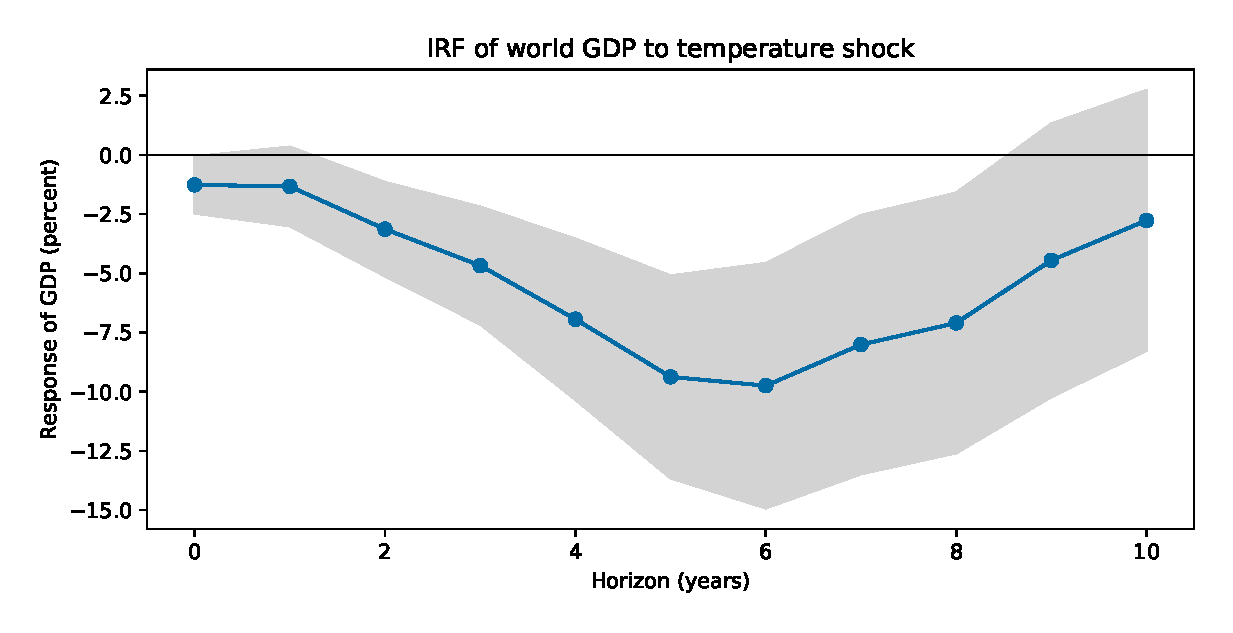
\includegraphics[width=\linewidth]{fig/bk_irf_contemp.eps}
\end{figure}
\end{frame}

\begin{frame}[fragile]
\scriptsize
\begin{verbatim}
# Estimate shock on full sample, using all controls
df['temp_anom_resid'] = sm.OLS(df['temp_anom'],
                               sm.add_constant(df[control_cols]),
                               missing='drop').fit().resid

# Summary statistics
print(df['temp_anom_resid'].describe())
\end{verbatim}
\bigskip
\normalsize
\textbf{Results:}
\scriptsize
\begin{verbatim}
count    5.800000e+01
mean    -6.849406e-15
std      9.938751e-02
min     -2.344768e-01
25%     -6.508441e-02
50%     -5.863778e-03
75%      6.166066e-02
max      2.645975e-01
Name: temp_anom_resid, dtype: float64
\end{verbatim}
\normalsize
Note: a 1 unit (i.e., 1$^\circ\text{C}$) climate shock is 4 $\times$ largest observed shock. Helpful for interpreting magnitudes in the IRF plots.
\end{frame}

\frame{
\begin{figure}
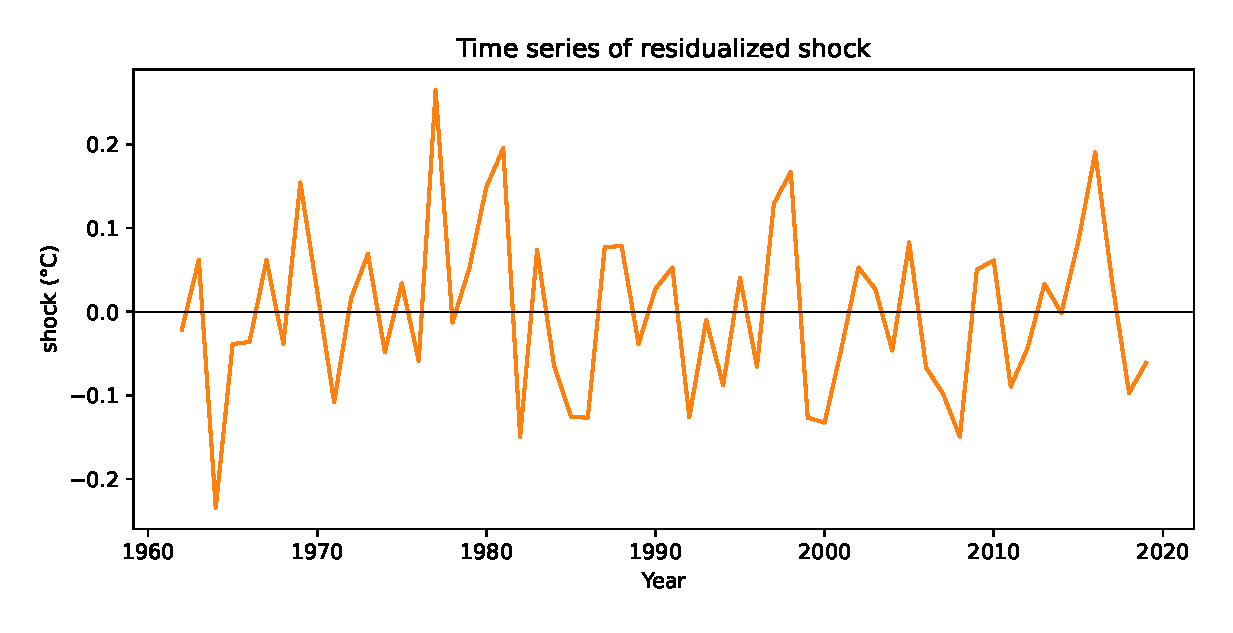
\includegraphics[width=0.8\linewidth]{fig/bk_shock.eps}
\end{figure}
\vspace{-\baselineskip}
\begin{figure}
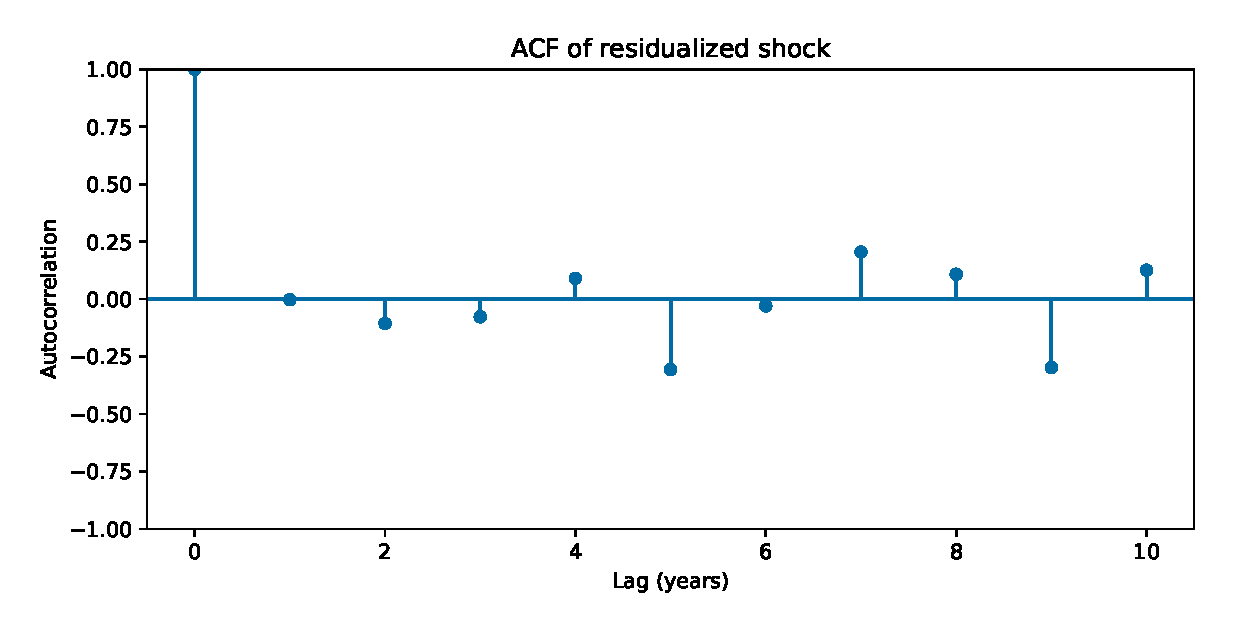
\includegraphics[width=0.8\linewidth]{fig/bk_shock_acf.eps}
\end{figure}
}

\frame{
\frametitle{Summary: LP with controls}
\begin{itemize}
\item Control for variables that are strong predictors of \emph{either} the outcome $y_t$ \emph{or} the impulse variable $x_t$.
\begin{itemize}
\item At a minimum, control for lags of $y_t$ and $x_t$.
\end{itemize}
\item Use economic theory or prior experience as a guide to select variables.
\item Use AIC to select lag length $p$.
\item Important to use lagged controls even if we directly observe a shock: increases efficiency and allows us to avoid Newey-West SE.
\item Use contemporaneous controls to remove confounding from other shocks. But must defend the timing assumptions!
\item Given controls, report diagnostics for residualized shock $\tilde{x}_t$.
\end{itemize}
}

\frame{
\frametitle{Importance of theory}
\begin{itemize}
\item LPs are easy to run but not always easy to interpret.
\item The residualized shock $\tilde{x}_t$ must correspond to something specific in relevant theoretical macro models.
\item Examples:
\begin{enumerate}
\item[\textcolor{green!50!black}{\ding{51}}] One could write a model of how climate interacts with the economy. One could imagine an external ``climate shock'' in such a model.
\item[\textcolor{red}{\ding{55}}] Suppose we ran an LP on $x_t = \text{GDP}_t$. What is this supposed ``GDP shock''? In most macro models, GDP is driven by multiple shocks: technology, monetary policy, ``animal spirits'', etc.
\end{enumerate}
\item Nobody will be impressed by your LP results if you don't have a concrete justification/interpretation for your identified shock.
\end{itemize}
}

\frame{
\frametitle{What did we learn?}
\begin{itemize}
\item SVMA model as a dynamic causal framework
\begin{itemize}
\item Changes to policy rules vs.\ shocks
\item IRF
\end{itemize}
\item LP estimation of IRFs
\begin{itemize}
\item Controls, lag length, SE
\item Residualized shock, shock diagnostics
\end{itemize}
\item Identification from timing restrictions
\end{itemize}
}

\frame{
\frametitle{Looking ahead}
\begin{itemize}
\item How important is our shock $\tilde{x}_t$ for the dynamics of $y_t$, relative to everything else that drives $y_t$?
\item What if $\tilde{x}_t$ is contaminated with measurement error?
\item Small-sample bias of LP and how to deal with it
\item How can we exploit panel data to estimate dynamic causal effects?
\end{itemize}
}

\end{document}
